\chapter{Experiments and Evaluation}\label{experiment}

In this section, we first present the performance of our proposed model in simulations and compare the results with the state-of-art models introduced in Ch.~\ref{preliminaries}. We then realize the proposed method wit our UAV flocking system and conduct real world experiments in both indoor and outdoor environments. We have also implemented a tracking algorithm with our system and compare their results in terms of flocking criteria.

\section{Simulation of Flocking Models}

We first show the influence of $\sigma$ and $\beta$ in (\ref{eq:proposed_ui}) to the convergence of the flock in Fig.~\ref{fig:sigma_beta}, where the averaged $\psi_{angle}$ (\ref{eq:psi_scal}) of twenty simulation results are illustrated with three cases. The more $\psi_{angle}$ gets close to one, the more convergent and aligned the flock is. As shown in the figure that the choice of $\sigma$ has little impact on the convergence rate compared with $\beta$. When $\beta\leq\frac{1}{2}$, the convergence of the whole flock is unconditional which is coincident with our assumption in Ch.~\ref{control_law}. We choose $\sigma=1$ and $\beta=0.25$ for all the following simulations and experiments. We compute the averaged results of $\psi_{angle}$ and relative distance from twenty simulations and plot them in Fig.~\ref{fig:multiple_agent}. We show that the cohesion, separation and alignment criteria still hold for our proposed model regardless of the number of total agents in the flock.

We compare our proposed flocking model with the ones in~\cite{Vicsek1995,CuckerSmale2007,CuckerDong2010} in Ch.~\ref{flocking} with 2, 3 and 4 agents respectively. The initial positions are illustrated in Fig.~\ref{fig:simulate_flocking} where the initial velocities are randomized. The positions of individual agents during the whole simulation are illustrated in Fig.~\ref{fig:N_pos} for reference. In Fig.~\ref{fig:N_scal} and Fig.~\ref{fig:N_mag}, we show that our proposed model converge as fast as those in~\cite{Vicsek1995,CuckerSmale2007,CuckerDong2010}. Especially, we show that the relative distance between neighboring agents in our proposed model is strictly bounded by the interval $(d_0^{\frac{1}{2}}, d_0^{\frac{1}{2}})$. Suppose certain minimum safety distance exists, such as $d_{safe}=0.8$ in Fig.~\ref{fig:N3_dis}, our proposed model could successfully avoided collision with neighboring agents.

\begin{figure}[H]
  \centering
  \subfigure[Case 1: $\sigma<1$ with $\sigma=0.5$]{\label{fig:sigma0_5}\includegraphics[width=0.49\textwidth]{figure/chapter_5/sigma0_5.png}}
  \subfigure[Case 2: $\sigma=1$]{\label{fig:sigma1}\includegraphics[width=0.49\textwidth]{figure/chapter_5/sigma1.png}}
  \quad
  \subfigure[Case 3: $\sigma>1$ with $\sigma=1.5$]{\label{fig:sigma1_5}\includegraphics[width=0.49\textwidth]{figure/chapter_5/sigma1_5.png}}
  \caption{Averaged $\psi_{angle}$ of twenty simulations of two agents w.r.t various $\sigma, \beta$. Their initial velocities are all randomized and nonzero.}\label{fig:sigma_beta}
\end{figure}

\begin{figure}[htb]
  \centering
  \subfigure[Average $\psi_{angle}$ of multiple agents with fixed $\sigma, \beta$]{\label{fig:multiple}\includegraphics[width=0.49\textwidth]{figure/chapter_5/multiple.png}}
  \subfigure[Average distance of multiple agents with fixed $\sigma, \beta$]{\label{fig:distance}\includegraphics[width=0.49\textwidth]{figure/chapter_5/distance.png}}
  \caption{Average $\psi_{angle}$ and relative distance of multiple agents with fixed $\sigma=1$ and $\beta=0.25$. Their initial velocity are all randomized and nonzero.}\label{fig:multiple_agent}
\end{figure}

\begin{figure}[H]
  \centering
  \subfigure[Two agents in a shape of straight line]{\label{fig:2_agents}\includegraphics[width=0.32\textwidth]{figure/chapter_5/2_agent.png}}
  \subfigure[Three agents in a shape of equilateral triangle]{\label{fig:3_agents}\includegraphics[width=0.32\textwidth]{figure/chapter_5/3_agent.png}}
  \subfigure[Four agents in a shape of diamond]{\label{fig:4_agents}\includegraphics[width=0.32\textwidth]{figure/chapter_5/4_agent.png}}
  \caption{Initial position settings of multi-agent flocking simulations in MATLAB.}\label{fig:simulate_flocking}
\end{figure}

\begin{figure}[H]
  \centering
  \subfigure[$N=2$ agents]{\label{fig:N2_scal}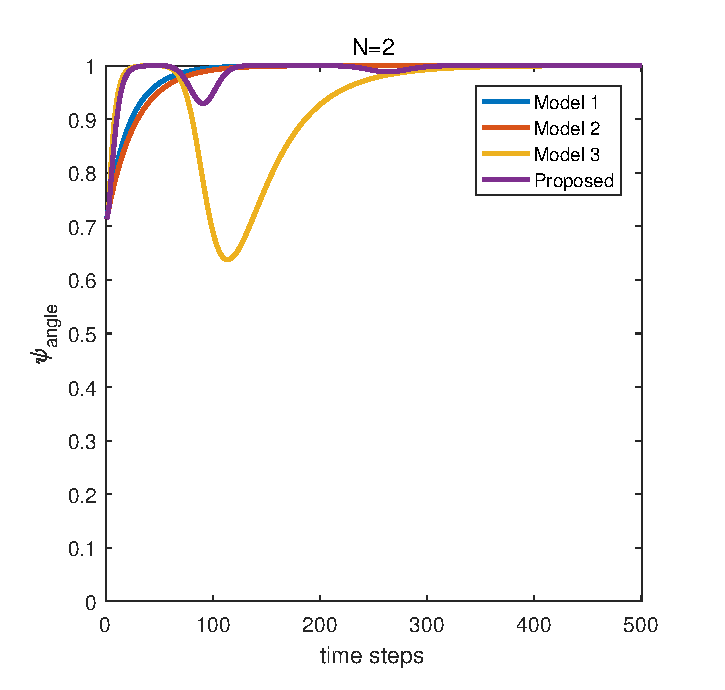
\includegraphics[width=0.49\textwidth]{figure/chapter_5/N2_scal.eps}}
  \subfigure[$N=3$ agents]{\label{fig:N3_scal}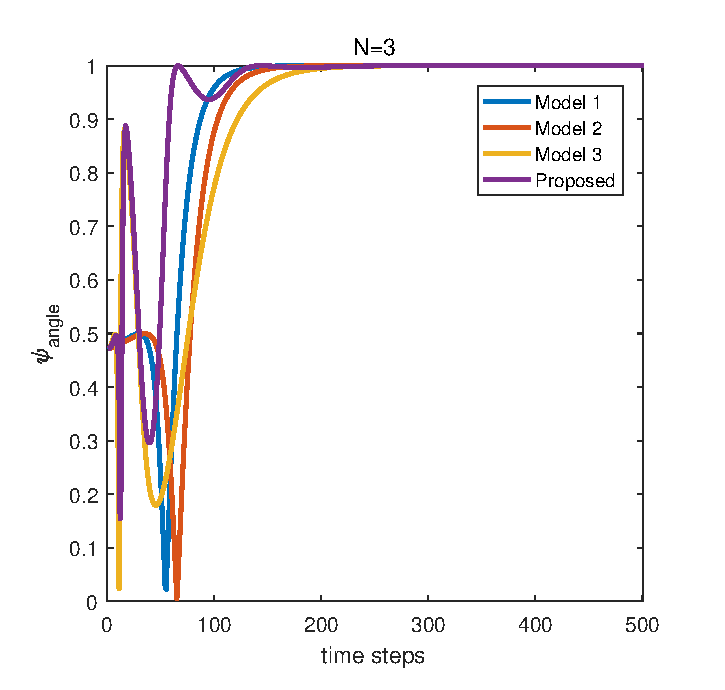
\includegraphics[width=0.49\textwidth]{figure/chapter_5/N3_scal.eps}}
  \quad
  \subfigure[$N=4$ agents]{\label{fig:N4_scal}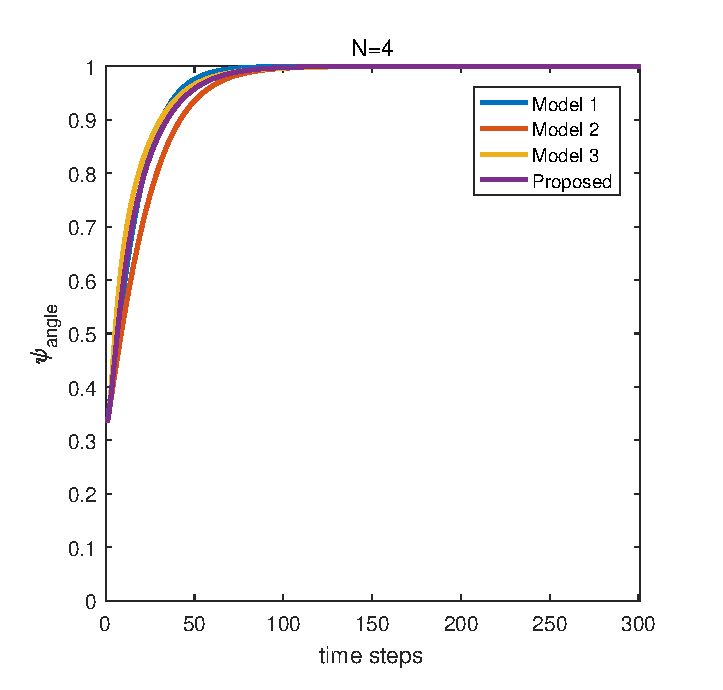
\includegraphics[width=0.49\textwidth]{figure/chapter_5/N4_scal.eps}}
  \caption{Convergence descriptors $\psi_{angle}$ of model 1 (\cite{Vicsek1995}), 2 (\cite{CuckerSmale2007}), 3 (\cite{CuckerDong2010}) and our proposed one.}\label{fig:N_scal}
\end{figure}

\begin{figure}[H]
  \centering
  \subfigure[$N=2$ agents]{\label{fig:N2_mag}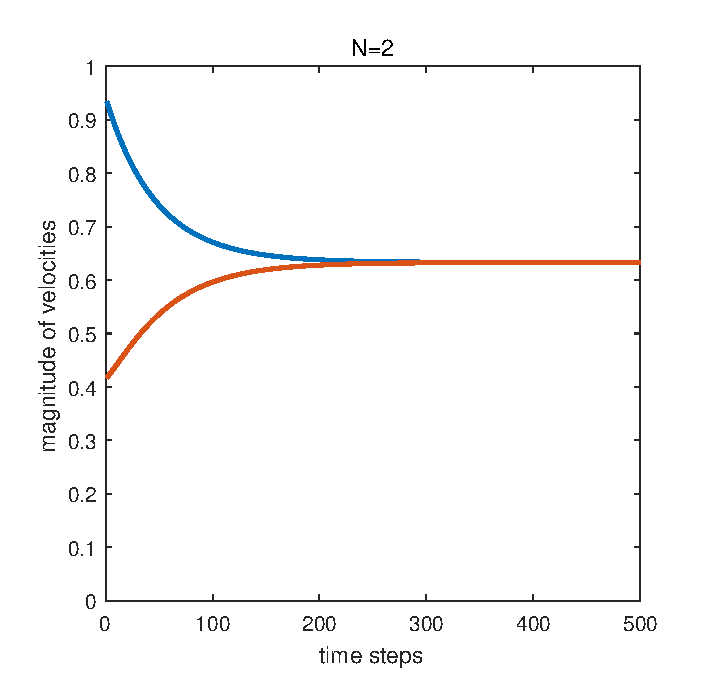
\includegraphics[width=0.49\textwidth]{figure/chapter_5/N2_mag.eps}}
  \subfigure[$N=3$ agents]{\label{fig:N3_mag}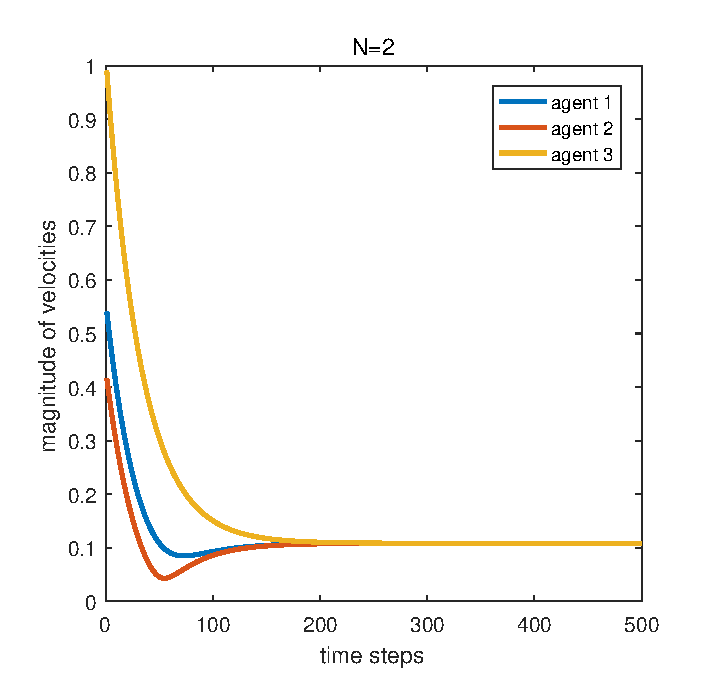
\includegraphics[width=0.49\textwidth]{figure/chapter_5/N3_mag.eps}}
  \quad
  \subfigure[$N=4$ agents]{\label{fig:N4_mag}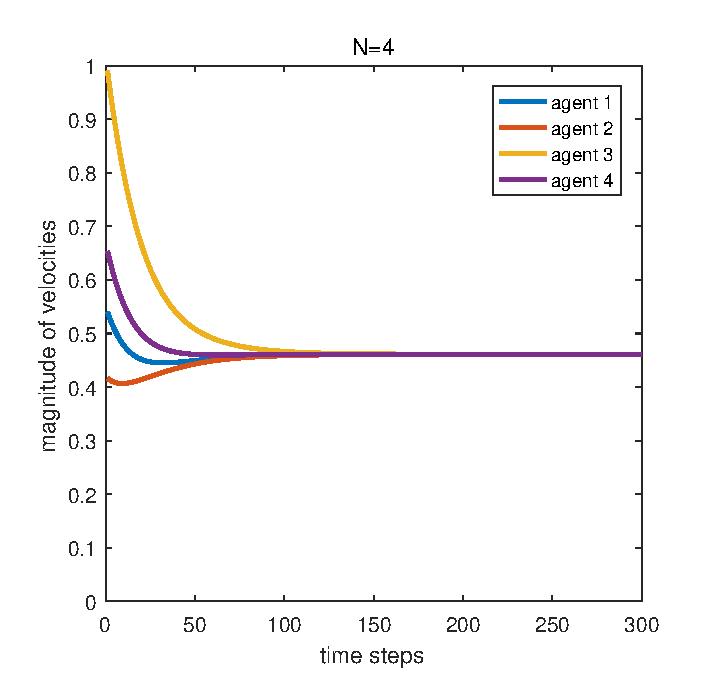
\includegraphics[width=0.49\textwidth]{figure/chapter_5/N4_mag.eps}}
  \caption{Magnitudes of agents' velocities of model 1 (\cite{Vicsek1995}), 2 (\cite{CuckerSmale2007}), 3 (\cite{CuckerDong2010}) and our proposed one.}\label{fig:N_mag}
\end{figure}

\begin{figure}[H]
  \centering
  \subfigure[$N=2$ agents.]{\label{fig:N2_dis}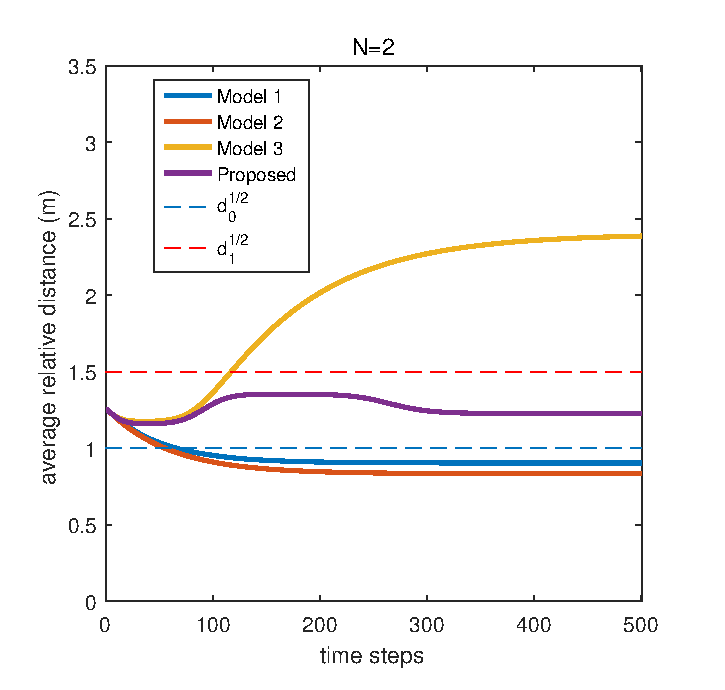
\includegraphics[width=0.49\textwidth]{figure/chapter_5/N2_dis.eps}}
  \subfigure[$N=3$ agents.]{\label{fig:N3_dis}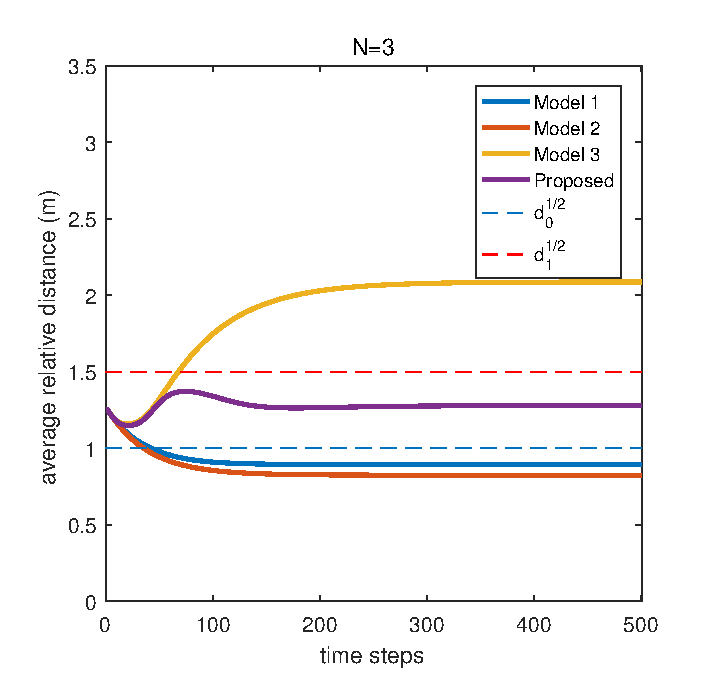
\includegraphics[width=0.49\textwidth]{figure/chapter_5/N3_dis.eps}}
  \quad
  \subfigure[$N=4$ agents.]{\label{fig:N4_dis}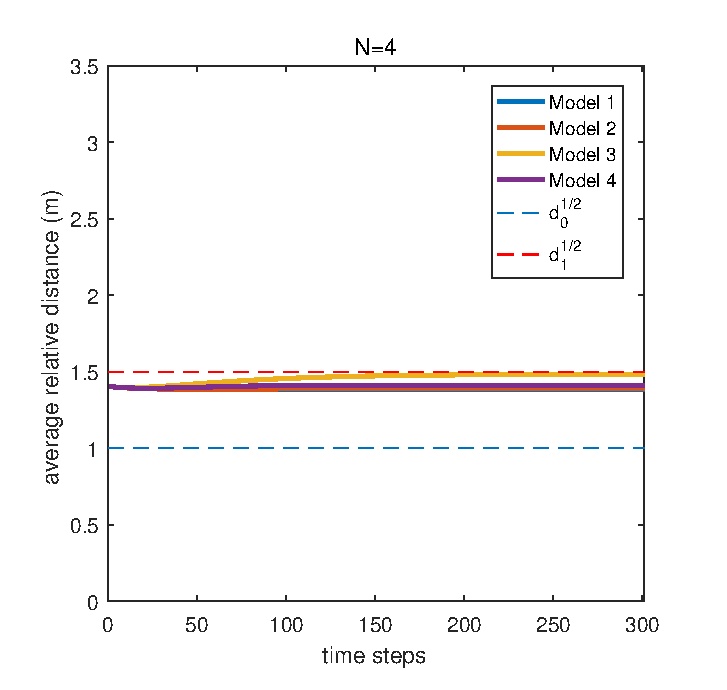
\includegraphics[width=0.49\textwidth]{figure/chapter_5/N4_dis.eps}}
  \caption{Average relative distances between neighboring agents. The blue and red dashed line indicate two boundaries $(d_0^{\frac{1}{2}}, d_1^{\frac{1}{2}})$ in our proposed model. Model 1, 2 and 3 are from~\cite{Vicsek1995},~\cite{CuckerSmale2007} and \cite{CuckerDong2010} respectively.}\label{fig:N_dis}
\end{figure}

\begin{figure}[H]
  \centering
  \subfigure[$N=2$ agents.]{\label{fig:N2_pos}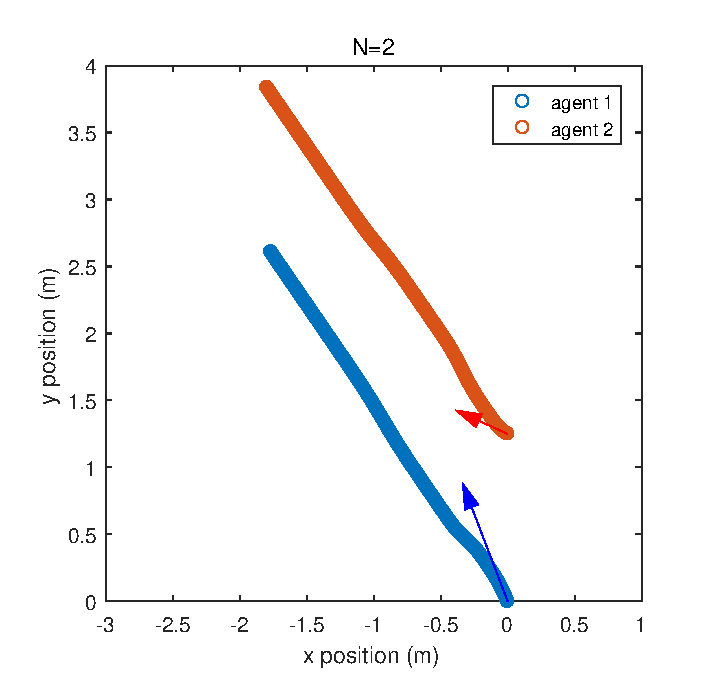
\includegraphics[width=0.49\textwidth]{figure/chapter_5/N2_pos.eps}}
  \subfigure[$N=3$ agents.]{\label{fig:N3_pos}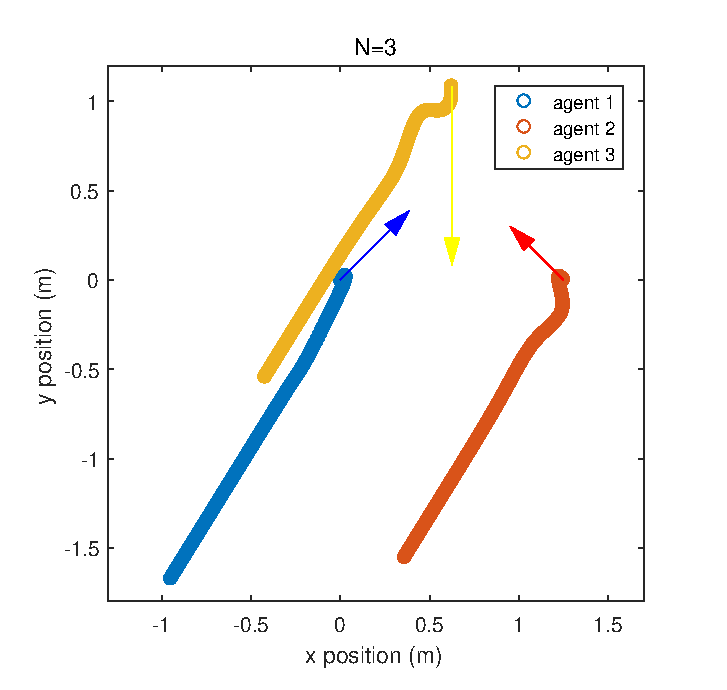
\includegraphics[width=0.49\textwidth]{figure/chapter_5/N3_pos.eps}}
  \quad
  \subfigure[$N=4$ agents.]{\label{fig:N4_pos}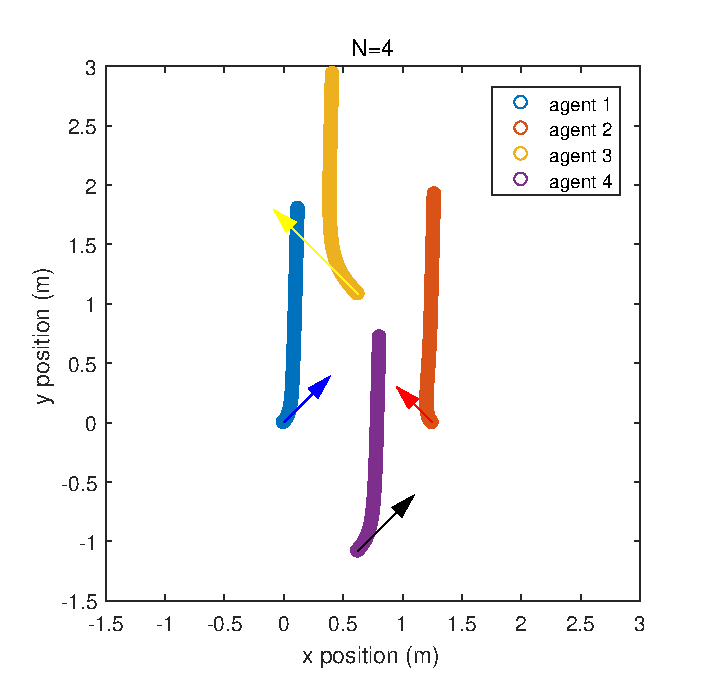
\includegraphics[width=0.49\textwidth]{figure/chapter_5/N4_pos.eps}}
  \caption{Motion simulations with initial velocities whose directions and magnitudes are indicated by corresponding arrows.}\label{fig:N_pos}
\end{figure}

\newpage

\section{Comparison with Formation Algorithm}\label{tracking}

We have reproduced the formation algorithm (\ref{eq:minT}, \ref{eq:minF}) in~\cite{Chenjing} and compared it with our flocking algorithm. The light green dots are the 3D positions of the leader calculated from captured images, a frame of which is shown in Fig.~\ref{fig:capture}.  As illustrated in Fig.~\ref{fig:track_plot}, the formation algorithm has maintained the relative displacement between follower UAV and leader UAV, however, it is clearly seen in Fig.~\ref{fig:position_plot} that the delay is inevitable.

\begin{equation}\label{eq:minT}
\min_{\hat{T}(\cdot)} \sum^{L}_{i=0} ||\hat{T}(t_i)-p_i||^2_2 + \lambda_t\int_{t_l}^{t_m} ||\hat{T}^{(2)}(t)||^2_2dt
\end{equation}

\begin{equation}\label{eq:minF}
\min_{f(\cdot)} \int_{t_0}^{t_m} ||f(t)-T_s(t)||^2_{2}dt + \lambda_f\int_{t_0}^{t_m} ||f^{(3)}(t)||^2_{2}dt\\
\end{equation}

\begin{figure}[htb]
  \centering
  \subfigure[The pink and green arrows indicate the leader's and follower's poses. The dark blue, light blue curves and the red one are the predicted path ${\hat{T}(t)}$, shifted path $T_s(t)$ and generated trajectory $f(t)$ respectively.]{\label{fig:rviz}\includegraphics[width=0.49\textwidth]{figure/chapter_5/rviz.png}}
  \subfigure[Image captured from follower's on-board camera. Green square indicates the recognized aruco code carried on leader UAV.]{\label{fig:capture}\includegraphics[width=0.49\textwidth]{figure/chapter_5/capture.png}}
  \caption{Formation algorithm in~\cite{Chenjing}.}\label{fig:rviz_capture}
\end{figure}

\subsection{Formation Performance}

\begin{figure}[H]
  \centering
  \subfigure[Position profiles of target and chaser UAVs. The blue and red lines are the x and y positions of the target UAV and the yellow and the purple lines are the x and y positions of the chaser UAV.]{\label{fig:position_plot}\includegraphics[width=0.49\textwidth]{figure/chapter_5/position_plot.png}}
  \subfigure[Relative distance between target and chaser UAVs. The desired shifted distance $d_s=1.5$ while the averaged relative distance $\bar{d}=1.39$.]{\label{fig:distance_plot}\includegraphics[width=0.49\textwidth]{figure/chapter_5/distance_plot.png}}
  \quad
  \subfigure[$\psi_{scal}$ of the tracking system.]{\label{fig:scal_plot}\includegraphics[width=0.49\textwidth]{figure/chapter_5/scal_plot.png}}
  \subfigure[Movement path reproduced in rviz.]{\label{fig:rviz_plot}\includegraphics[width=0.49\textwidth]{figure/chapter_5/rviz_plot.png}}
  \caption{Plots of tracking algorithm.}\label{fig:track_plot}
\end{figure}

\section{Realization of Proposed Model}

In this section, we demonstrate that our flocking system is able to operate in both indoor and outdoor GPS-denied environments. All the experiment settings are identical, where the follower UAV takes off first and hovers at desired height, waiting for the leader, then the leader UAV takes off and the control authority of follower switches to autonomous mode to begin flocking. The desired $u_i$ is updated when a newer photo comes in and in each time interval (roughly 0.1 s) the latest $u_i$ is being executed. The initial take off position of follower UAV is 1.5 m behind the leader UAV to match the requirement ($d_0<||x_i-x_j||^2<d_1$) with $d_0=1, d_1=8, K=1, k=2, \alpha=1$ and $\beta=0.25$ in Ch.~\ref{control_law}. The maximum acceleration and velocity of follower UAV are set to $a_{max}=2.5 m/s^2$ and $v_{max}=0.5 m/s$ for safety reasons. In each experiment we show their position profile, relative distance, $\psi_{angle}$ plot and their movement path reproduced in rivz. Due to the measurement noise, light condition and lack of ground truth, spikes appear randomly in all figures. We have shown that the trend of slope in $\psi_{angle}$ plot is in accordance with that in position plot, the follower UAV is able stay flocking with the leader and the reaction of follower is rapid.

\subsection{Indoor Environment}

We have conducted two experiments in the indoor environment. We first let the leader UAV moves purely along the x-axis (positive pointing forward) and then y-axis (positive pointing left), with their results being illustrated in Fig.~\ref{fig:x_indoor} and Fig.~\ref{fig:y_indoor}. Noted that $\psi_{scal}$ plot is calculated with the data all obtained from follower UAV.

\begin{figure}[htb]
  \centering
  \subfigure[Position profiles of leader and follower UAVs. The yellow and purple lines are the x and y positions of the leader UAV and the blue and the red lines are the x and y positions of the follower UAV.]{\label{fig:x_indoor_position}\includegraphics[width=0.49\textwidth]{figure/chapter_5/x_indoor_position.png}}
  \subfigure[Relative distance between leader and follower UAVs in x axis.]{\label{fig:x_indoor_distance}\includegraphics[width=0.49\textwidth]{figure/chapter_5/x_indoor_distance.png}}
  \quad
  \subfigure[$\psi_{angle}$]{\label{fig:x_indoor_scal}\includegraphics[width=0.49\textwidth]{figure/chapter_5/x_indoor_scal.png}}
  \subfigure[Movement path reproduced in rviz.]{\label{fig:x_indoor_rviz}\includegraphics[width=0.49\textwidth]{figure/chapter_5/x_indoor_rviz.png}}
  \caption{Flocking in x-axis.}\label{fig:x_indoor}
\end{figure}

\begin{figure}[htb]
  \centering
  \subfigure[Position profiles of leader and follower UAVs. The yellow and purple lines are the x and y positions of the leader UAV and the blue and the red lines are the x and y positions of the follower UAV.]{\label{fig:y_indoor_position}\includegraphics[width=0.49\textwidth]{figure/chapter_5/y_indoor_position.png}}
  \subfigure[Relative distance between leader and follower UAVs in y axis.]{\label{fig:y_indoor_distance}\includegraphics[width=0.49\textwidth]{figure/chapter_5/y_indoor_distance.png}}
  \quad
  \subfigure[$\psi_{angle}$]{\label{fig:y_indoor_scal}\includegraphics[width=0.49\textwidth]{figure/chapter_5/y_indoor_scal.png}}
  \subfigure[Movement path reproduced in rviz.]{\label{fig:y_indoor_rviz}\includegraphics[width=0.49\textwidth]{figure/chapter_5/y_indoor_rviz.png}}
  \caption{Flocking in y-axis.}\label{fig:y_indoor}
\end{figure}

\subsection{Outdoor Environment}

In the outdoor environment, we let the leader UAV moves in the xy-plane. Due to the outdoor wind condition that the follower UAV has deviated a little from desired position, moreover, the relative distance between two UAVs is kept within the desired boundary.

\begin{figure}[htb]
  \centering
  \subfigure[Position profiles of leader and follower UAVs. The yellow and purple lines are the x and y positions of the leader UAV and the blue and the red lines are the x and y positions of the follower UAV.]{\label{fig:xy_outdoor_position}\includegraphics[width=0.49\textwidth]{figure/chapter_5/xy_outdoor_position.png}}
  \subfigure[Relative distance between leader and follower UAVs. The light blue and red dashed line indicate the $d_0^{\frac{1}{2}}, d_1^{\frac{1}{2}}$ respectively. ]{\label{fig:xy_outdoor_distance}\includegraphics[width=0.49\textwidth]{figure/chapter_5/xy_outdoor_distance.png}}
  \quad
  \subfigure[$\psi_{angle}$]{\label{fig:xy_outdoor_scal}\includegraphics[width=0.49\textwidth]{figure/chapter_5/xy_outdoor_scal.png}}
  \subfigure[Movement path reproduced in rviz.]{\label{fig:xy_outdoor_rviz}\includegraphics[width=0.49\textwidth]{figure/chapter_5/xy_outdoor_rviz.png}}
  \caption{Flocking in xy-plane.}\label{fig:xy_outdoor}
\end{figure}

\newpage
